\documentclass[11pt,a4paper]{article}
\usepackage[T1]{fontenc}
\usepackage{lmodern}
\usepackage[margin=25mm]{geometry}
\usepackage{amsmath,amssymb,amsthm,mathtools}
\renewcommand{\qedsymbol}{\textnormal{\small Q.E.D.}}
\usepackage{graphicx,booktabs,array,tabularx}
\usepackage{microtype}
\usepackage{caption}
\usepackage[numbers,sort&compress]{natbib}
\usepackage{xurl}
\usepackage{xcolor}
\usepackage[colorlinks=true,linkcolor=blue!40!black,citecolor=blue!40!black,urlcolor=blue!40!black]{hyperref}
\hypersetup{pdftitle={Verified affine constructions, recursive families, and incidence bounds for Kobon triangles},pdfauthor={Alejandro Zarzuelo Urdiales}}
\newtheorem{theorem}{Theorem}[section]
\newtheorem{lemma}[theorem]{Lemma}
\newtheorem{proposition}[theorem]{Proposition}
\newtheorem{corollary}[theorem]{Corollary}
\theoremstyle{definition}
\newtheorem{definition}[theorem]{Definition}
\theoremstyle{remark}
\newtheorem{remark}[theorem]{Remark}
\newcommand{\K}{K}
\newcommand{\Ks}{K_{\mathrm s}}
\newcommand{\G}{G}
\newcommand{\B}{B}
\newcommand{\N}{\mathbb N}
\newcommand{\R}{\mathbb R}
\newcommand{\Z}{\mathbb Z}
\newcommand{\floor}[1]{\left\lfloor#1\right\rfloor}
\newcommand{\ceil}[1]{\left\lceil#1\right\rceil}
\newcommand{\lean}[1]{{\small\nolinkurl{#1}}}
\newcommand{\proofref}[3]{\href{https://github.com/alejandrozu/kobon-proof/blob/2d69a71e32d3eaa59399b0e5bc61720ec3b00ac8/#1\#L#2}{#3}}
\DeclareMathOperator{\sgn}{sgn}
\setlength{\emergencystretch}{2em}
\captionsetup{font=small,labelfont=bf}
\setcounter{topnumber}{3}
\renewcommand{\topfraction}{0.9}
\renewcommand{\textfraction}{0.08}
\renewcommand{\floatpagefraction}{0.75}
\graphicspath{{figures/}}
\title{Verified constructions and incidence bounds\\for Kobon triangles}
\author{Alejandro Zarzuelo Urdiales}
\date{3 October 2026}
\begin{document}
\maketitle
\begin{abstract}
We give explicit real-line constructions and a Lean development for lower and upper bounds on triangular cells. A phase correction and change of affine chart refine the F\"uredi--Pal\'asti all-order guarantee to $\lfloor n(n-3)/3\rfloor+1+(n\bmod2)$ for $n\ge4$. We complete geometric iteration of a compatible Bartholdi--Blanc--Loisel seed, including the boundary invariant needed for even companions: at $q=10\cdot2^t$, the certified counts are $(q^2-4)/3$ on $q+1$ lines and that number plus $q/2$ on $q+2$ lines. A verified total envelope retains all earlier certificates and improves the previous verified envelope at infinitely many orders. Formal geometric upper bounds place both recursive families within one triangle of the classical simple bounds. We also establish actual multiplicity and clean-line incidence identities, a prescribed-grid obstruction, and an exterior-extension resource limitation. Exact larger-seed calculations and restricted upper arguments are reported with their remaining proof obligations. The advances concern constructions and verification; no new numerical record or solution of the unrestricted problem is claimed.
\end{abstract}
\section{Introduction and relation to previous work}

Let $\K(n)$ count the largest possible number of bounded triangular cells formed by $n$ distinct straight lines in $\R^2$, allowing parallel pairs and multiple intersections. Let $\Ks(n)$ restrict to \emph{simple} arrangements, with no parallel pair and no three concurrent lines. Thus $\K(n)\ge\Ks(n)$. A triangular cell is a component of the complement whose closure is a nondegenerate triangle; arbitrary intersecting triples are not counted.

F\"uredi--Pal\'asti's trigonometric arrangements imply the all-order affine bound $\B(n)=\ceil{n(n-3)/3}$ for $n\ge3$; its ceiling form is explicit in Erickson, and related affine counts appear in Felsner--Kriegel~\cite{furedipalasti1984,erickson1999,felsnerkriegel1999}. Our first complete construction refines its constant term.

\begin{theorem}[Uniform affine refinement]\label{j:main}
For every $n\in\N$, $\Ks(n)\ge\G(n)$, where $\G(n)=0$ for $n<3$, $\G(3)=1$, and
\begin{equation}\label{j:G}
 \G(n)=\floor{\frac{n(n-3)}3}+1+(n\bmod2),\qquad n\ge4.
\end{equation}
For $n\ge4$, the gains $\G(n)-\B(n)$ in residue classes $0,1,\ldots,5$ modulo six are $1,1,0,2,0,1$.
\end{theorem}

Section~\ref{j:construction} constructs actual real lines and triangular interiors; its general Lean proof uses only the standard logical axioms. The gain is at most two and leaves the leading terms $n^2/3-n$ unchanged. Related constants already occur in projective F\"uredi--Pal\'asti counts. We claim an explicit affine refinement and its verification, without establishing first numerical priority for the formula.

Stronger special families predate this work. Forge--Ram\'irez Alfons\'in give a projective construction yielding optimal affine orders $2\cdot2^t+1$~\cite{forge1998}. Bartholdi--Blanc--Loisel (BBL) give compatible doubling and straight-line optimal families at $6\cdot2^t+1$ and $14\cdot2^t+1$~\cite{bbl2008}. Parpalak--Utkin establish the straight-line family $18\cdot2^t+1$~\cite{parpalakutkin2026}, with $108\cdot4^t-1$ triangles. Taking a maximum and adding distant lines already yields further all-order guarantees. All-order validity therefore differs from numerical optimality at every order.

The classical comparison polynomial is $U_{\mathrm T}(n)=\floor{n(n-2)/3}$; Cl\'ement--Bader discuss unrestricted upper bounds and residue refinements~\cite{clementbader2007}. Blanc proves the stronger simple even bound~\cite{blanc2011}
\begin{equation}\label{j:blanc}
 \Ks(n)\le U_{\rm e}(n):=\floor{\frac{n(2n-5)}6},\qquad n\ge4\text{ even}.
\end{equation}
Nonsimple $14$-line examples with $54$ triangles exceed $U_{\rm e}(14)=53$; simplicity cannot be suppressed. We now formalize these two \emph{simple} geometric bounds and combine them with completed BBL iteration to obtain one-triangle windows at both parities (Section~\ref{jfam:section}). This upgrades the earlier manuscript's polynomial comparisons to actual upper theorems and its finite recursive checkpoints to infinite geometric families.

The March proposal~\cite{zarzuelo2026} sought a general one-line successor rule. Its unrestricted recurrence remains unproved; its historical finite conclusions have independent certificates. The present account also retains exterior-extension geometry and its boundary-resource obstruction, exact finite gains, multiplicity-sensitive arguments and smoothing diagnostics. Recent SAT and straightening work~\cite{savchuk2025}, coordinate releases~\cite{maiorana2026,parpalakutkinGallery2026}, and pseudoline enumeration~\cite{parpalakutkinEnumeration2026} supply attributed inputs and methods. Our contribution includes exact obstruction certificates for one prescribed tangent grid; it does not turn pseudoline enumeration into an unproved straight-line classification. The companion research manuscript~\cite{zarzueloFull2026} gives full proofs, all individual certificates, historical comparisons and unsuccessful searches.

\section{The uniform affine construction}\label{j:construction}

Write $\ell:a_\ell x+b_\ell y=c_\ell$ and $f_\ell(x,y)=a_\ell x+b_\ell y-c_\ell$. For nonparallel supports put
\[
 D_{\ell m}=a_\ell b_m-b_\ell a_m,\qquad
 (X_{\ell m},Y_{\ell m})=(c_\ell b_m-b_\ell c_m,a_\ell c_m-c_\ell a_m).
\]
Their intersection is $p_{\ell m}=(X_{\ell m},Y_{\ell m})/D_{\ell m}$. The polynomial
\[
 O(r;\ell,m)=(a_rX_{\ell m}+b_rY_{\ell m}-c_rD_{\ell m})D_{\ell m}
            =f_r(p_{\ell m})D_{\ell m}^2
\]
has the sign of the actual affine evaluation. An increasing nonconcurrent triple is \emph{certified} if its three values $O(r;i,j),O(r;i,k),O(r;j,k)$ have a common weak sign for every arrangement line $r$.

\begin{lemma}\label{j:cell}
In an arrangement without parallel pairs, a certified triple has a nonempty triangular interior equal to a strict sign cell. Different increasing certified triples have disjoint interiors; each is a bounded triangular cell.
\end{lemma}
\begin{proof}
The vertices are noncollinear. Every test line has one weak sign on their convex hull and a strict sign inside: vanishing at an interior convex combination would force vanishing at all three vertices. Conversely, the supporting inequalities give positive barycentric coordinates. Thus the interior is exactly one strict sign cell. These cells are convex components of the complement. Equal interiors have the same three open sides and hence the same increasing support triple.
\end{proof}
Lean proves the geometric sign-cell equality and disjointness; the connected-component interpretation follows by the last elementary topological observation. Rational coordinates allow denominator clearing to integer tests.

Use the F\"uredi--Pal\'asti family
\begin{equation}\label{j:trig}
 \ell(\theta):\quad \sin\theta\,x+\cos\theta\,y=\sin(3\theta).
\end{equation}
Its determinant is $\sin(u-v)$, and direct expansion gives
\begin{equation}\label{j:sign}
 O(\ell(w);\ell(u),\ell(v))
 =4\sin^2(u-v)\sin(w-v)\sin(w-u)\sin(u+v+w).
\end{equation}
For $\theta_i=(i+a)\pi/n$, $0\le i<n$, choose triples with
\begin{equation}\label{j:residues}
 i+j+k\equiv\begin{cases}n-1,n-2\pmod n,&a=1/2,\\0,n-1\pmod n,&a=1/6.\end{cases}
\end{equation}
The arrangements are simple. A selected sum is $s\pi\pm\pi/(2n)$; at an external test index $r$, the sign in~\eqref{j:sign} is
$(-1)^s\sgn(r-i)\sgn(r-j)\sgn(r-k)$, independent of the pair. Supporting indices cause no conflict. Thus all selected triples are certified.

For each residue, $i+j+k=b$ has $n^2$ ordered solutions. The three equality sets $i=j$, $i=k$, $j=k$ each have $n$ elements. Using two residues, excluding repetitions and dividing by six gives $\B(n)$ for the half phase.
\begin{lemma}[Phase correction]\label{j:phase}
The phase $a=1/6$ gives at least $\floor{n(n-3)/3}+1$ cells for $n\ge3$.
\end{lemma}
\begin{proof}
For residue zero, the three equality sets meet at $(0,0,0)$, so their union has size at most $3n-2$. The other residue costs at most $3n$. Hence $6T\ge2n^2-6n+2$; rounding gives the assertion.
\end{proof}

The projective chart $(x,y)\mapsto(x/(h-x),y/(h-x))$ transforms a line into $\Phi_h(a,b,c)=(ha-c,hb,c)$. If $E$ denotes the first factor defining $O$, then
\begin{align}
 D(\Phi_h\ell,\Phi_hm)&=h(h-x_{\ell m})D(\ell,m),\notag\\
 E(\Phi_hr;\Phi_h\ell,\Phi_hm)&=h^2E(r;\ell,m),\notag\\
 O(\Phi_hr;\Phi_h\ell,\Phi_hm)&=h^3(h-x_{\ell m})O(r;\ell,m).\label{j:covariance}
\end{align}
A cut avoiding vertices preserves simplicity. The sign multiplier preserves old triangles on its retained side and reverses the sign at an exposed vertex on the opposite side.

\begin{lemma}[Exposed caps]\label{j:caps}
For odd $n\ge3$, a chart of the half-phase arrangement has $\B(n)+1$ cells. If $n=6k+3\ge9$, a chart has $\B(n)+2$ cells.
\end{lemma}
\begin{proof}[Proof outline, with explicit supports]
The intersection abscissa is $\cos(2u)+\cos(2v)+\cos(2u+2v)$. Put $c_n=1+2\cos(\pi/n)$. The pair $(0,n-1)$ is uniquely rightmost, at $c_n$; take $h>0$ just below it. For $n=2m+1$, the triple $(0,m,2m)$ is absent from the old list and has the opposite weak sign only at that pair. Formula~\eqref{j:covariance} corrects it, retaining every old cell.

For $n=6k+3=3m$, the pairs $(m-1,m)$ and $(2m-1,2m)$ are exactly the leftmost vertices, both at $-c_n/2$. The discrete cosine comparison is proved in the linked two-cap source and detailed in the companion manuscript. Taking $h<0$ just above them corrects exactly the exposed signs of $(2k,2k+1,5k+2)$ and $(k,4k+1,4k+2)$. They are distinct and absent from the old list. Every old selected triangle survives. All assertions, including exposure, are symbolic Lean theorems.
\end{proof}

\begin{figure}[tb]
\centering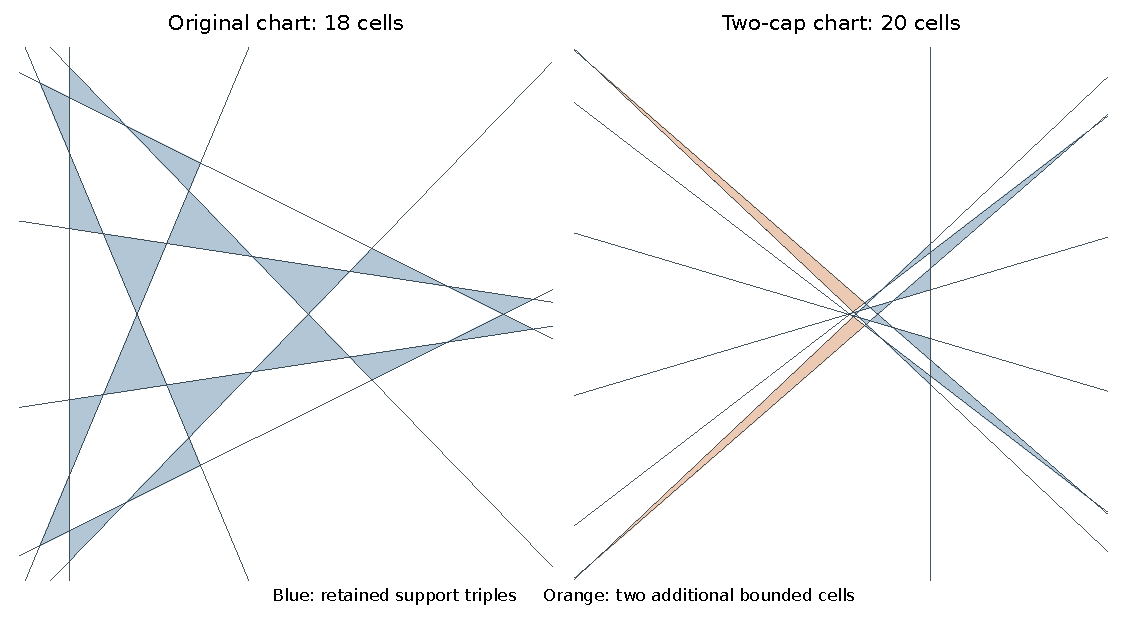
\includegraphics[width=.74\linewidth]{affine-chart.pdf}
\caption{Exact rational illustration of the two-cap change at $n=9$: 18 old cells survive and two become bounded. This gives $\G(9)=20$, below the known optimum 21. The general theorem uses real trigonometric coordinates; panels are independently rescaled.}\label{j:fig-chart}
\end{figure}

\begin{proof}[Proof of Theorem~\ref{j:main}]
For even orders use the shifted phase. If $n$ is odd and not divisible by three, $\B(n)+1=\floor{n(n-3)/3}+2$; use one cap. For odd multiples of three at least nine use two caps. A triangle handles $n=3$. The residue calculation gives the stated gains.
\end{proof}
The exact remaining gap is
\begin{equation}\label{j:gap}
 U_{\mathrm T}(n)-\G(n)
 =\floor{n/3}+\mathbf1_{n\equiv2\ (3)}-1-(n\bmod2),\qquad n\ge4.
\end{equation}
This is an independent construction at each order, not a successor chain from an arbitrary optimal seed.

\section{Exterior extensions and their boundary resource}
\label{jext:section}

Exterior addition has precedents in BBL and Blanc~\cite{bbl2008,blanc2011}.
The contribution here is an explicit geometric certificate, a quantitative
defect formulation for both parities, and an obstruction to repeatedly
demanding the full gain proposed in March~\cite{zarzuelo2026}.

Let $A$ be a simple $n$-line arrangement, $n\ge3$, with equations $f_i=0$ and
vertices $p_{ij}$.  A linear functional $w$ is admissible if it is nonzero
on every line direction.  At $p_{ij}$ choose support directions $u_i,u_j$
with $w(u_i)=w(u_j)=1$.  Call the pair \emph{visible} if, for every old
line $f_k=0$, the numbers
\[
 f_k(p_{ij}),\quad Df_k(u_i),\quad Df_k(u_j)
\]
have one common weak sign.  This condition certifies an empty unbounded
wedge using only old data.

\begin{theorem}[Verified exterior realization]
\label{jext:visible}
If $A$ contains $T$ distinct certified triangles and $c$ distinct pairs
visible from an admissible $w$, adjoining $w(x)=H$, where
$H>\max_{i<j}w(p_{ij})$, gives a simple arrangement with at least $T+c$
triangles.
\end{theorem}
\begin{proof}
The new line is nonparallel to every support, misses all old vertices,
and lies beyond every old bounded cell.  Thus simplicity and old triangles
are preserved.  A visible pair has new vertices
$p_{ij}+(H-w(p_{ij}))u_i$ and $p_{ij}+(H-w(p_{ij}))u_j$.
Their affine evaluations are
$f_k(p_{ij})+(H-w(p_{ij}))Df_k(u)$, so all three vertices have one weak
sign against every old line.  The triangle is nondegenerate and empty.
Distinct pairs give distinct new support triples, all containing the
new line and hence distinct from the old triples.
\end{proof}
This is \proofref{Kobon/Exterior.lean}{164}{\lean{Exterior.extension}}, a real-coordinate Lean theorem with
no parity restriction or assumed future count.

Write $T=t(A)$, $d=n(n-2)-3T$, and let $b$ count unbounded two-sided cells.
The quantity $d$ counts unused bounded elementary segments: a segment
in a simple arrangement supports at most one triangle.

\begin{proposition}[Boundary-defect extension]
\label{jext:defect}
For $n\ge3$, define
\begin{equation}
 g(n,T)=\ceil{\frac{n-1}{2n}\max\{3,\,3T-n(n-3)\}}.
 \label{jext:gain}
\end{equation}
Then $\Ks(n)\ge T$ implies $\Ks(n+1)\ge T+g(n,T)$.
\end{proposition}
\begin{proof}
There are $2n$ free rays, of which $2b$ belong to wedges.  At an unpaired
ray's endpoint $L\cap M$, both incident segments of $M$ are bounded.
They cannot both support triangles, since those triangles would share
the unique bounded segment of $L$ starting there.  Charge this ray to
an unused segment of $M$.  Each unused segment receives at most two
endpoint charges, giving $b+d\ge n$.  Convex-hull vertices of the finite
intersection set supply at least three wedges, so $b\ge\max\{3,n-d\}$.

The two rays of a wedge are consecutive in cyclic direction order.
Among the $2n$ admissible normal sectors, each wedge is visible in
exactly $n-1$: positivity selects $n$ consecutive oriented directions.
Thus some sector sees at least $\ceil{(n-1)b/(2n)}$ wedges.  Apply
Theorem~\ref{jext:visible}.  The expression is nondecreasing in $T$,
so a lower count can replace the witness's actual count.
\end{proof}
The cyclic count and defect arithmetic are formalized.  The universal
ray-charging and geometric cyclic-data extraction remain manuscript
proofs; the proposition is not claimed as an end-to-end Lean theorem.

If $n=2m+1$ and $d\le2$, then $b\ge2m-1$.  Averaging forces at least
$m$ visible wedges, since
$2m(2m-1)>(4m+2)(m-1)$; no sector can contain more than $m$ disjoint
ray pairs.  Hence every such odd input admits the full gain $m$.
For either parity the exact full-gain test is that some sector contains
$\floor{n/2}$ wedge pairs.  The defect rule itself can be iterated
without assuming this stronger condition persists.

Repeated exterior additions have a finite boundary resource.  If $b_r$
is the wedge count and $c_r$ the gain, each new triangle consumes an
old wedge.  No new free ray appears at an old vertex, and new wedges
can use only the two free rays of the added line.  Therefore
\begin{equation}
 b_{r+1}+c_r\le b_r+2,\qquad
 \sum_{j<r}c_j\le b_0+2r-3.
 \label{jext:budget}
\end{equation}
Quadratically accumulating full gains cannot continue indefinitely.
For the saved $49:767$ seed, $b_0=47$; gains $24$ and $25$ in two
exterior steps would leave at most two wedges, contradicting $b\ge3$.
This does not refute a recurrence for maxima using reconstruction.

One recorded exterior chain has gains $24,23,2,2$, giving
$49{:}767\to50{:}791\to51{:}814\to52{:}816\to53{:}818$.
Its capacities describe those arrangements, not upper bounds for $\K$.
The companion manuscript plots the exact resource evolution.


Conditionally, $F(n+1)\ge F(n)+\floor{n/2}$ yields
\[
 F(n)\ge F(s)+\floor{(n-1)^2/4}-\floor{(s-1)^2/4}.
\]
The recurrence remains unproved for $\K$.  Nevertheless its $49$-seed
numerical target is independently unconditional:
\begin{equation}
 \K(n)\ge\floor{(n-1)^2/4}+191\qquad(n\ge49).
 \label{jext:49}
\end{equation}
Lean proves this from the finite 49/50 witnesses and the classical
baseline for $n\ge51$; it does not construct a nested full-gain chain.

\section{Completed recursive families and a total envelope}
\label{jfam:section}

The doubling mechanism belongs to BBL~\cite{bbl2008}. The new formalization closes the actual geometric invariant and, separately, the visibility needed for every even companion.

\begin{theorem}[Verified BBL step]\label{jfam:doubling}
Let $q=4r\ge20$, $0<\varepsilon<\tan(\pi/(2q))$, and $t_j=\tan(j\pi/q)$. Take $Y_0:y=0$ and $L_j:y=m_j(x-a_j)$ on the ordered grid
\[
 (a_j)=(-t_{q/2-1},\ldots,-t_1,-\varepsilon,\varepsilon,t_1,\ldots,t_{q/2-1}).
\]
Assume simplicity, all $q-1$ cells $(Y_0,L_j,L_{j+1})$, positive central-apex height, and $T$ distinct certified triangles. Then $\Ks(2q+1)\ge T+q^2$.
\end{theorem}
\begin{proof}[Geometric mechanism]
With $\beta_i=-\pi/2+(i+1/2)\pi/q$, add the $q$ lines
\[
 y=\kappa\bigl(\sin(2\beta_i)+\delta\cot\beta_i\bigr)(x-\tan\beta_i).
\]
Exact intersection identities give crossing order first for sufficiently small $\delta>0$, then $\kappa>0$. The row count gives $2\binom{q+1}{2}-q=q^2$ mixed triangles. Old triangles off $Y_0$ persist; alternating caps replace the noncentral triangles on it, and the central triangle survives. Simplicity, disjoint support lists and their actual sign certificates are proved, not assumed future properties.
\end{proof}

Our eleven-line compatible realization uses $x-v_jy=a_j$, where
\[
 (v_j)=\tfrac1{10}(15,-2,14,1,4,-4,5,-3,12,-5).
\]
For every real $0<\varepsilon\le10^{-5}$, it has 32 triangles, nine distinguished triangles and five pairs visible from $(10,-13)$. The count is inherited from a Honma-based input described by Savchuk~\cite{savchuk2025}; the uniform tangent-grid realization is the certificate contribution. A separate 21-line uniform seed has 132 triangles, 19 distinguished triangles and ten visible pairs. It starts the $r\ge5$ induction; the eleven-line case is supplied separately.

\begin{theorem}[Actual infinite families]\label{jfam:recursive}
For every integer $t\ge0$, put $q=10\cdot2^t$ and $T_q=(q^2-4)/3$. There are simple real-line arrangements satisfying
\begin{equation}\label{jfam:families}
 \Ks(q+1)\ge T_q,\qquad \Ks(q+2)\ge T_q+q/2.
\end{equation}
Both inequalities are complete Lean theorems.
\end{theorem}
\begin{proof}[Invariant and iteration]
A seed records actual grid equations, simplicity, all consecutive distinguished triangles, positive central apex, and a duplicate-free certified triangle list. The geometric step returns all this data. Explicit mutually inverse label maps sort its new grid; triangle-support transport preserves validity and list length. Uniform availability on some interval $0<\varepsilon<\eta$ is retained, so induction applies at every finite depth.

For the even branch the record additionally contains an admissible normal, actual visible pairs and a clean rightmost ray. Projection-order transfer and a sufficiently small common choice of pencil scale preserve this boundary data. Starting with $(r,T,V)=(5,132,10)$, the proved transformation is
\[
 (r,T,V)\longmapsto(2r,T+(4r)^2,V+2r).
\]
It yields $T_q=(q^2-4)/3$ and $V=q/2$. Apply the verified exterior realization once at each depth. The eleven-line seed supplies $t=0$.
\end{proof}
The quantifier is: for every finite depth there is a positive parameter interval and actual arrangements on it. No single fixed $\varepsilon$ is asserted to work at all depths. The proof does not assert a successive $+1$ chain or applicability to an arbitrary optimal input.

\begin{theorem}[One-triangle simple windows]\label{jfam:windows}
For the same $q$,
\[
 T_q\le\Ks(q+1)\le T_q+1,\qquad
 T_q+q/2\le\Ks(q+2)\le T_q+q/2+1.
\]
\end{theorem}
\begin{proof}
The actual simple bounds proved in Section~\ref{jup:section} give
$\floor{(q+1)(q-1)/3}=T_q+1$ and
$\floor{(q+2)(2q-1)/6}=T_q+q/2+1$.
Combine with Theorem~\ref{jfam:recursive}.
\end{proof}
The upper halves use only standard Lean axioms. The existence halves inherit four finite native checks from the 21-line seed, and six for the even family; the recursive geometry itself uses standard axioms. These are formal optimality windows for simple arrangements, not improved numerical literature records or even upper bounds for arbitrary multiple intersections.

Let $C(n)$ be the largest saved finite certificate at order $n$, or zero, and retain the earlier verified envelope
\begin{equation}\label{j:envelope}
 L(n)=\max\{\G(n),C(n)\}\le\K(n).
\end{equation}
Define $R(n)=T_q$ if $n=q+1$, $R(n)=T_q+q/2$ if $n=q+2$, for $q=10\cdot2^t$, and $R(n)=0$ otherwise.
\begin{theorem}[Improved verified all-order bound]\label{j:new-envelope}
For every $n\in\N$,
\begin{equation}\label{j:new-envelope-formula}
 \K(n)\ge H(n):=\max\{L(n),R(n)\}\ge L(n).
\end{equation}
The final inequality is strict at both $n=10\cdot2^{t+5}+1$ and $n=10\cdot2^{t+5}+2$ for every $t\ge0$.
\end{theorem}
\begin{proof}
Each branch has an actual witness. Lean implements $R$ by a finite maximum over indices at most $n$, which includes every matching branch. The retained catalog has no order above 195, so $L(n)=\G(n)$ there. Direct arithmetic gives
\begin{equation}\label{j:new-gains}
 T_q-\G(q+1)=\floor{q/3}-2,\qquad
 T_q+q/2-\G(q+2)=q/2-\floor{q/3}-2.
\end{equation}
Both are positive from $q=320$ onward.
\end{proof}
The gains at 321 and 322 are 104 and 52; at 641 and 642 they are 211 and 105. This compares complete \emph{verified repository envelopes}, not every construction in the literature. The new theorem proves existence at $321{:}34132$, $322{:}34292$, $641{:}136532$ and $642{:}136852$ without retroactively certifying every archived coordinate file. Earlier checkpoints $81{:}2132$, $82{:}2172$, $161{:}8532$, $162{:}8612$ remain included. At small family orders the retained catalog can be stronger, for example $12{:}38$, $21{:}133$, $22{:}143$, $41{:}533$ and $42{:}553$.

\begin{figure}[tb]
\centering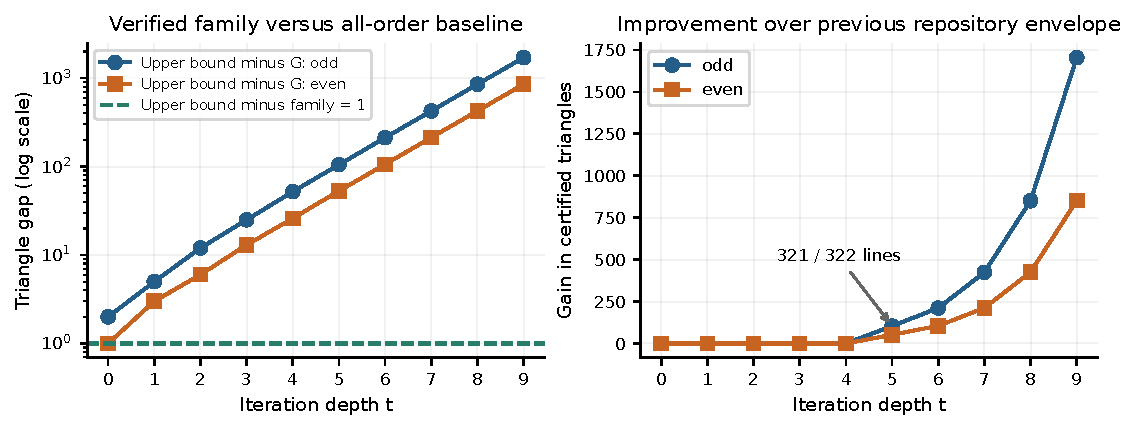
\includegraphics[width=.91\linewidth]{recursive-envelope.pdf}
\caption{Verified recursive counts compared with the previous all-order envelope and the classical simple upper benchmarks. The new existence theorem improves the retained bound on two infinite sparse sets. Both family branches have upper-minus-lower gap one; other orders retain their previous bound. These are not numerical-record claims.}\label{j:fig-gap}
\end{figure}

Known dyadic optimal constructions retain Forge--Ram\'irez Alfons\'in attribution; our corrected five-line normalization has five triangles, three distinguished triangles and two visible pairs on $0<\varepsilon\le10^{-5}$. An independent exact interval check reproduces 107 triangles and 17 distinguished triangles for the Parpalak--Utkin 19-line input on $0<\varepsilon\le10^{-3}$. Neither becomes a new unconditional family theorem here. At $q=4\cdot2^t$ and $18\cdot2^t$, the inherited odd formulas are $(q^2-1)/3$ and $q^2/3-1$; the ordinary boundary-defect argument gives full-gain even companions. Complete uniform 33- and 49-line seeds would give stronger formal families, but their full finite Lean checks remain unfinished (Section~\ref{j:verification}).

\section{Actual incidence bounds and remaining core geometry}
\label{jup:section}

Here the lines are pairwise nonparallel. Multiple points are allowed except in explicitly simple statements. The completed Lean extraction applies to any finite injective certified triangle family, including a proper subset of all triangular cells; unused and shared edges are counted relative to that family.

Let $t_r$ count $r$-fold vertices. The core consists of those with $r\ge3$; set
\[
 q=\sum_{r\ge3}t_r,\quad I=\sum_{r\ge3}rt_r,\quad
 S=\sum_{r\ge3}r(r-2)t_r,\quad\delta=n(n-2)-3T.
\]
Let $h$ count lines meeting the core, $E$ bounded elementary segments, $U$ unused segments, and $D_1,D_2$ shared sides with one and two core endpoints. An actual shared side cannot have two ordinary endpoints. Pair counting, consecutive-intersection extraction and the capacity of an edge to border at most two triangle interiors now give complete Lean identities
\begin{equation}\label{jup:identity}
 E=n(n-2)-S,\qquad3T=E-U+D_1+D_2,\qquad
 \delta=S+U-D_1-D_2.
\end{equation}
Actual core incidences also give $D_2+h\le I$, $D_2\le\binom q2$, and $2S-7I+15q\ge0$.

\begin{lemma}[Actual clean-line charging]\label{jup:clean}
For even $n\ge4$, $n-h\le2U+D_1$. Consequently
\begin{equation}\label{jup:budget}
 2\delta\ge n+2S-h-3D_1-2D_2.
\end{equation}
\end{lemma}
\begin{proof}[Completed geometric extraction]
A clean line avoids the core and has $n-1$ distinct crossings. Choose a common open half-plane containing another transverse intersection on each crossing line. Consecutive-intersection order supplies bounded transverse pieces there. If every such piece had triangle degree one, the triangles would pair the clean line's crossings; uniqueness of consecutive segments makes this a partition into pairs. Its odd cardinality $n-1$ is impossible. Hence a bounded transverse piece is unused or shared. Its clean-line endpoint is ordinary, so a shared piece has precisely one core endpoint. An unused segment receives at most two endpoint charges and a one-core shared segment at most one. The actual charge map and its fibers are extracted in Lean, yielding the inequality. Equation~\eqref{jup:identity} then gives~\eqref{jup:budget}.
\end{proof}
This completion is distinct from the exterior \emph{ray}-charging gap in Proposition~\ref{jext:defect}. Nonparallelism is used to obtain the transverse intersections: three parallel vertical lines and one horizontal line would invalidate the same clean-line statement.

\begin{theorem}[Formal classical simple bounds]\label{jup:simple}
Every simple $n$-line certificate witness satisfies $3T\le n(n-2)$ for $n\ge2$, and $6T\le n(2n-5)$ for even $n\ge4$.
\end{theorem}
\begin{proof}
The core is empty, so $S=D_1=D_2=h=0$ and $\delta=U\ge0$. In the even case Lemma~\ref{jup:clean} gives $2U\ge n$. Rearranging proves both inequalities, including their floor forms.
\end{proof}
These are formalizations of classical simple upper bounds, including Blanc's even polynomial~\cite{blanc2011}; they are not new unrestricted estimates. Together with Theorem~\ref{jfam:recursive}, they prove the windows stated there.

\begin{lemma}[Local fan bounds]\label{jup:fan}
At an $r$-fold core point, let $d_1,d_2$ count shared incident rays ending respectively at ordinary and core vertices. The actual cyclic fan satisfies
\[
 d_1\le2r-3,\qquad3d_1+d_2\le6r-6.
\]
An extremal fan with $d_1=2r-3$ has every sector triangular and exactly $d_2=3$. Thus $d_2\le2$ implies $d_1\le2r-4$.
\end{lemma}
\begin{proof}[Local mechanism]
There cannot be $r-1$ consecutive ordinary-ended shared rays: successive opposite supports coincide, forcing a line to meet an opposite pair of rays and hence the center. Window counting gives the first bound. Analysis of the missing sectors shows that equality forces the full triangular fan and three core-ended rays. Combining this with $d_1+d_2\le2r$ proves the other conclusions.
\end{proof}
The local geometric interfaces and this sharper equality analysis are complete Lean results. With $e_v$ the indicator of an extremal fan, they also yield
\begin{equation}\label{jup:sharp-fan}
 3d_1+d_2\le6r-8+2e_v.
\end{equation}
A supported boundary core cannot be extremal under the supplied fan/endpoint maps. Two full triple fans cannot be adjacent under the explicit common-edge matching. Extracting all these cyclic fans and matches from arbitrary whole arrangements remains unfinished. If that extraction supplies the summed fan inequality and $e=\sum_v e_v$, the complete conditional arithmetic theorem gives
\begin{equation}\label{jup:exceptional}
 2\delta\ge n+2S-7I+8q+D_2-2e.
\end{equation}
This retains the shared-core-edge correction. The following older restricted claims retain their ordinary-proof status.

\begin{theorem}[Restricted upper estimates: manuscript geometry]\label{jup:upper}
For even nonparallel arrangements, the global fan argument gives
\begin{equation}\label{jup:weighted}
 2\delta\ge n+\sum_{r\ge3}(2r^2-11r+6)t_r.
\end{equation}
If there are at most two core points, then
\begin{equation}\label{jup:two-core}
 T\le\floor{n(n-5/2)/3}+1.
\end{equation}
The defects for zero and one core point satisfy $\delta\ge n/2$ and $\delta\ge n/2-1$ respectively.
\end{theorem}
\begin{proof}
Summing $3d_1+d_2\le6r-6$ gives $3D_1+2D_2\le6I-6q$; with $h\le I$, use~\eqref{jup:budget}. If $q\le2$, every core has $d_2\le1$, so $D_1\le2I-4q$. Since $D_2\le1$ and $h\le I-D_2$, one obtains
$2\delta\ge n+\sum(2r^2-11r+12)t_r-D_2\ge n-3q-D_2\ge n-7$.
Parity improves this to $n-6$. For $q=0,1$ the same argument has $D_2=0$ and rounds as stated.
\end{proof}
A nonnegative total weight in~\eqref{jup:weighted} gives the simple even polynomial; in particular this holds when every core multiplicity is at least five. Triple and quadruple weights are $-9,-6$, so this does not solve the arbitrary-core case. The two-core bound is attained within its stated class at $8,14,26,50$ lines by attributed witnesses with $15,54,204,792$ triangles~\cite{maiorana2026,parpalakutkinGallery2026}. The new three-core arithmetic theorem gives $T\le\floor{n(2n-5)/6}+2$ when its fan premises are supplied. It is conditional, not a completed unrestricted geometric bound.

Shared sides cannot be discarded. The six lines $x=0$, $y=0$, $x+y=3$, $x-y=0$, $2x+y=3$, $x+2y=3$ have six triangular cells and six shared radial sides at $(1,1)$, with $d_1=d_2=3$. Their exact Lean certificate contradicts only a literal local incidence interpretation of a shared-pair assertion in Cl\'ement--Bader~\cite{clementbader2007}, not its final upper theorem.
\begin{figure}[tb]
\centering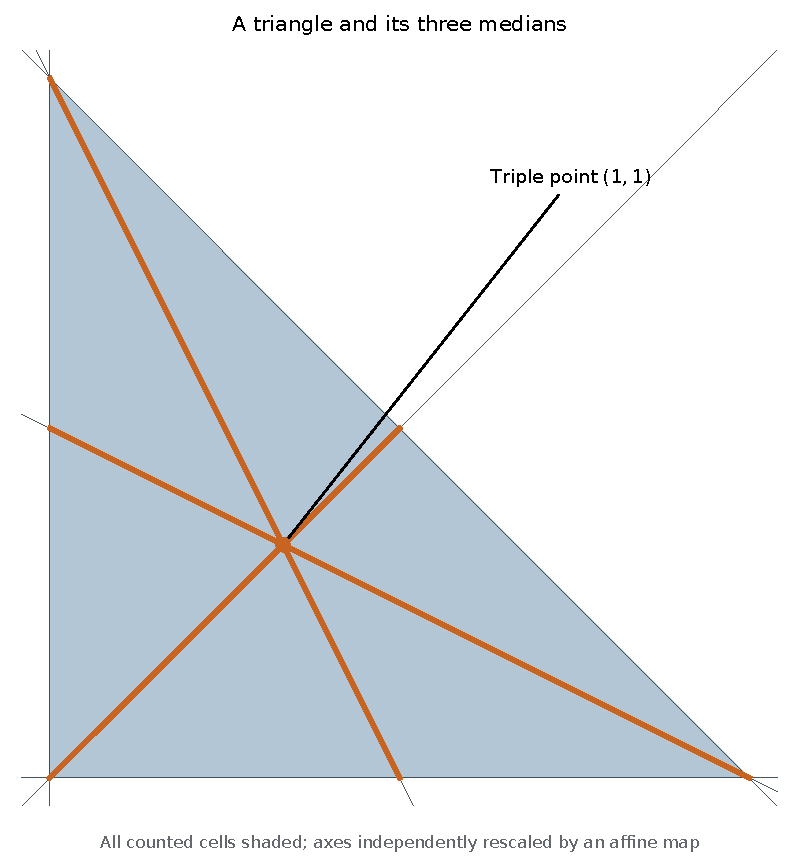
\includegraphics[width=.43\linewidth]{shared-fan.pdf}
\caption{The verified triangle-and-medians example: six cells, three ordinary-ended and three core-ended shared sides at the central triple point. This distinction controls the incidence budget.}\label{jup:figure}
\end{figure}

Exact smoothing diagnostics also survive unchanged. The four local resolutions of the retained Maiorana $14{:}54$ input count $52,52,53,52$ cells. For 132 recorded gallery resolutions at orders $8,14,20,26,32,38,50$, the respective best nearby simple counts are $14,51,114,203,313,448,791$. Fixed nonzero determinant signs and the resolved triple signs control sufficiently small perturbations. These finite exact computations refute nondecreasing, and even universal loss-at-most-one, smoothing for the specified input types. The sign-stability interpretation is an ordinary argument; the data do not bound every simple arrangement at those orders.

\section{Finite results, exact obstructions, and verification}\label{j:verification}

The release retains 138 coordinate identities, 104 simple, with original credits. Table~\ref{j:finite} preserves the individual historical inequalities and all eleven later affine materializations. The companion catalog lists every input and its source.
\begin{table}[tb]
\centering\small
\begin{tabular}{@{}llp{.33\linewidth}@{}}
\toprule
Order(s) & Certified counts, in order & Role\\\midrule
$28,30,34$ & $238,275,357$ & Historical inequalities\\
$44$ & $608$ & Simple optimum\\
$39,47,48$ & $470,691,721$ & Earlier retained count plus one\\
$51,53,54,55$ & $818,885,919,955$ & Earlier retained count plus one\\
$59,60,99,195$ & $1103,1141,3170,12482$ & Earlier retained count plus one\\
\bottomrule
\end{tabular}
\caption{Selected exact simple witnesses. The increases are relative to earlier project certificates, not asserted global records. All orders 3--60 and all 138 coordinate identities are in the companion evidence.}\label{j:finite}
\end{table}

The March-associated $28{:}238$, $30{:}275$, $34{:}357$ inequalities now have independent certificates; the archived extension proof remains incomplete~\cite{zarzuelo2026,oeisA006066}. Earlier literature overlaps are explicit: $30{:}275$ is in BBL, and $34{:}357$ follows from the older perfect 33-line construction and exterior addition~\cite{bbl2008,forge1998}. The exact $43{:}587\to44{:}608$ construction combined with the now-formal simple upper theorem gives $\Ks(44)=608$, not $\K(44)=608$. The earlier proposed value $q^2/3+q+1$ at $n=q+3$, $q=6\cdot2^t$, is superseded by $\G(q+3)=q^2/3+q+2$.

Two independent rational counters support the finite catalog. Reproduced external inputs include all fifteen Maiorana $14{:}54$ configurations and ten Parpalak--Utkin gallery witnesses, including $26{:}204$ and $50{:}792$~\cite{maiorana2026,parpalakutkinGallery2026}. Exact projective face censuses for the saved 81- and 161-line examples equal 2132 and 8532, their bounded counts: a chart change alone cannot improve these two fixed arrangements.

\paragraph{A prescribed-grid obstruction.}
In reciprocal coordinates $x-v_i y=a_i$, required orientation signs become strict linear inequalities in the $v_i$. Positive linear dependencies certify infeasibility. Lean proves this Farkas-type soundness principle and the exact coefficient field
\[
 t=\tan(\pi/20),\qquad t^4-4t^3-14t^2-4t+1=0,\qquad3/20<t<17/100,
\]
including all nine positive grid tangents as power-basis expressions.
\begin{proposition}\label{j:obstruction}
The ten specified orientation signs linked in \proofref{Kobon/BBLGridObstruction.lean}{263}{the exact obstruction statement} cannot occur on the prescribed 20-intercept tangent grid, for any real $\varepsilon$ and arbitrary real reciprocal slopes.
\end{proposition}
This representative obstruction is fully in Lean with standard axioms. A separate exact verifier checks 3,765 polynomial dependencies and 15,060 reflected/reoriented variants, covering all $236\cdot21=4,956$ supplied Euclidean-class/distinguished-support cases for $0<\varepsilon<1/2{,}000{,}000$. The input classification and its completeness are attributed to Parpalak--Utkin~\cite{parpalakutkinEnumeration2026}; their enumeration is not rerun or formalized here. Subject to that external classification, the corpus excludes a perfect 21-line seed on this specific saturated grid and interval. The earlier 18-projective-representative scan omitted affine charts and has been replaced by this corrected coverage. An exact external interval calculation also proves radius-$10^{-3}$ intercept robustness for the representative's eleven used intercepts. Other grids and larger seeds remain possible.

\paragraph{A larger compatible seed, with a remaining finite check.}
A new exact external 49-line uniform certificate uses rational reciprocal slopes of denominator $10^{10}$ on the 48-intercept tangent grid. For every $0<\varepsilon\le1/100$ it has 767 triangles, 47 distinguished triangles, positive central apex and 24 pairs visible from $(1,-2)$. Two independent exact counters agree at the rational midpoint. Actual rational bounds for the 23 positive tangents are proved in Lean. The full exported seed's direction, simplicity, support and visibility checks pass an independent exact Python audit, but its complete Lean finite validation was stopped without completion. Hence its prospective recursive counts
\begin{equation}\label{j:exact49}
 \begin{array}{ll}
 n=48\cdot2^t+1:&768\cdot4^t-1,\\
 n=48\cdot2^t+2:&768\cdot4^t+24\cdot2^t-1
 \end{array}
\end{equation}
are not unconditional theorems of the active library. The odd orders are the $s=t+3$ tail of BBL's established $6\cdot2^s+1$ family~\cite{bbl2008}. Likewise, the verified generic 33-line-seed implication gives $(1024\cdot4^t-1)/3$ and that value plus $16\cdot2^t$, but the needed uniform finite seed remains a draft; the numerical family retains Forge--Ram\'irez Alfons\'in attribution~\cite{forge1998}.

Bounded searches found no numerical record: deletion, mixed-integer line selection, singular insertions and straightening are logged with their limits. For example, all 9,180 tested 17-line vertex-pair chords reached at most 93 triangles at order 18; 407,253 tested 43-line pairs reached 607 at order 44. Two 39-line straightening searches certified 353 and 358 triangles, respectively; neither is a record or a nonstretchability result. These experiments motivate certificates and alternate grids, not impossibility claims.

\paragraph{Proof release and remaining work.}
The mathematical snapshot is pinned at \texttt{2d69a71}; it uses Lean 4.31.0 and Mathlib~\cite{lean4,mathlib}. All 270 build targets and 375 active sources passed, with 5,241 audited theorem declarations: 4,405 depend only on standard logical axioms, and 836 have finite native-check dependencies. These are implementation counts, not numbers of discoveries. Active proofs have no \lean{sorry}, \lean{admit}, custom geometric axioms or unsafe declarations. Native certificates additionally trust the compiler/runtime path of \lean{native_decide}. Five new exact external replay audits passed; they remain external computations. The \href{https://github.com/alejandrozu/kobon-proof/actions/runs/37056093885}{successful release CI} and result map link every status to evidence.

The next mathematical task is whole-arrangement cyclic-fan extraction and shared-edge matching, followed by a justified aggregate bound for arbitrary triple and quadruple cores. A recorded graph deduction makes the next target concrete: if exceptional triple cores have three distinct core neighbors and no two are adjacent, incidence counting gives $3e\le D_2$. If every exceptional fan is triple, equation~\eqref{jup:exceptional} then gives $2\delta\ge n+2S-7I+8q+e$ and $6\delta\ge3n+6S-21I+24q+D_2$. These unformalized corollaries require the missing degree/matching interface; they are not stronger than retaining the exact $D_2-2e$ correction, nor do they improve an unrestricted numerical upper bound. Larger compatible seeds and a generalized grid offer lower-bound routes. The arbitrary successive $+1$ recurrence remains separate and unproved. The source, experiments and expanded manuscript~\cite{zarzueloRepository,zarzueloFull2026} preserve both successful and unsuccessful work. Computer algebra, exact search and AI assistance contributed to the development; the stated evidence, rather than generated assertions, supports each conclusion.

\section*{Result-to-proof index}\label{j:proof-index}

All source links below are pinned to revision \texttt{2d69a71}. \textbf{K} denotes proofs using standard Lean axioms; \textbf{N} also inherits finite \texttt{native\_decide} checks. \textbf{P} marks an ordinary manuscript proof with formal components; \textbf{E} marks exact external computation. A linked conditional theorem proves only its stated implication. The \href{https://github.com/alejandrozu/kobon-proof/blob/main/manuscripts/2026-10-03/shared/proof_map.md}{complete result map} gives every statement, hypothesis, source anchor and individual certificate, including all 138 coordinate identities and the unfinished branches.

\begingroup\small\renewcommand{\arraystretch}{1.09}
\noindent\begin{tabularx}{\linewidth}{@{}>{\raggedright\arraybackslash}p{.25\linewidth}>{\raggedright\arraybackslash}X@{}}
\toprule
Result & Immutable Lean source and scope\\\midrule
Theorem~\ref{j:main}; \eqref{j:G}, \eqref{j:gap} &
\proofref{Kobon/Universal.lean}{26}{Affine all-order construction}, \proofref{Kobon/Universal.lean}{72}{gains}, \proofref{Kobon/Universal.lean}{90}{gap}: K.\\
Lemma~\ref{j:cell} & \proofref{Kobon/Cells.lean}{486}{Sign-cell equality}, \proofref{Kobon/Cells.lean}{453}{disjointness}: K for nonparallel arrangements; component interpretation P.\\
Lemmas~\ref{j:phase}, \ref{j:caps} & \proofref{Kobon/ShiftedFurediPalasti.lean}{274}{Phase correction}, \proofref{Kobon/FurediPalastiWrap.lean}{191}{one cap}, \proofref{Kobon/FurediPalastiTwoCaps.lean}{282}{two caps}: K.\\
Theorem~\ref{jext:visible} & \proofref{Kobon/Exterior.lean}{164}{Actual exterior realization}: K from certified visible pairs.\\
Proposition~\ref{jext:defect}; \eqref{jext:budget} & \proofref{Kobon/BoundaryExtension.lean}{79}{Defect arithmetic}, \proofref{Kobon/Iteration.lean}{105}{iteration budget}: K conditional; global boundary geometry P.\\
Target~\eqref{jext:49} & \proofref{Kobon/AllN.lean}{504}{Unconditional numerical target}: N, no nested-chain claim.\\
Theorem~\ref{jfam:doubling} & \proofref{Kobon/BBLDoubling.lean}{15}{Actual BBL step}: K with compatible seed.\\
Parameterized seeds & \proofref{Kobon/SeedFamily.lean}{115}{Eleven}, \proofref{Kobon/BBLSeed21Normalized.lean}{91}{twenty-one}, \proofref{Kobon/BBLSeed21Visible.lean}{44}{visibility}; seed finite trust disclosed.\\
Theorem~\ref{jfam:recursive}; \eqref{jfam:families} & \proofref{Kobon/BBLRecursiveSeed.lean}{61}{Closed seed step}, \proofref{Kobon/BBLInfinite.lean}{46}{odd induction}, \proofref{Kobon/BBLEvenInfinite.lean}{43}{even induction}: K generic; \proofref{Kobon/BBLVerifiedFamilies.lean}{24}{odd}, \proofref{Kobon/BBLVerifiedFamilies.lean}{51}{even}: N unconditional.\\
Theorem~\ref{jfam:windows} & \proofref{Kobon/BBLFamilyOptimality.lean}{29}{Odd window}, \proofref{Kobon/BBLFamilyOptimality.lean}{35}{even window}: N existence, K universal upper halves.\\
Theorem~\ref{j:new-envelope}; \eqref{j:new-gains} & \proofref{Kobon/RecursiveEnvelope.lean}{51}{All-order envelope}: N; \proofref{Kobon/RecursiveEnvelope.lean}{73}{strict infinite gains}: K comparison.\\
Identity~\eqref{jup:identity}; Lemma~\ref{jup:clean} & \proofref{Kobon/UpperEdgeInventory.lean}{345}{Actual defect}, \proofref{Kobon/UpperCleanCharging.lean}{100}{actual charge map}: K, no counting/charging premise.\\
Theorem~\ref{jup:simple} & \proofref{Kobon/UpperSimpleOptimality.lean}{70}{Simple upper floor}, \proofref{Kobon/UpperEvenSimpleOptimality.lean}{69}{even floor}: K actual geometry.\\
Lemma~\ref{jup:fan}; \eqref{jup:sharp-fan} & \proofref{Kobon/UpperFan.lean}{171}{Full-fan equality}, \proofref{Kobon/UpperFan.lean}{227}{weighted bound}, \proofref{Kobon/UpperTripleFan.lean}{156}{triple incompatibility}: K with explicit local/matching interface.\\
Theorem~\ref{jup:upper}; \eqref{jup:exceptional} & \proofref{Kobon/CleanLineBudget.lean}{73}{Weighted arithmetic}, \proofref{Kobon/CleanLineBudget.lean}{58}{two cores}, \proofref{Kobon/UpperCoreBudget.lean}{47}{core-edge correction}, \proofref{Kobon/UpperCoreBudget.lean}{58}{three cores}: conditional K; global fan extraction P/pending.\\
Figure~\ref{jup:figure}; Table~\ref{j:finite} & \proofref{Kobon/SharedFan.lean}{51}{Six shared sides}: K; \proofref{verification/certificate-index.json}{1}{individual certificate index}: finite N where recorded.\\
Proposition~\ref{j:obstruction} & \proofref{Kobon/BBLGridObstruction.lean}{263}{Actual tangent-grid obstruction}: K for one sign system; full 236-class corpus E plus external classification.\\
Larger seeds; smoothing & \proofref{Kobon/BBLTangent48Bounds.lean}{1}{Actual tangent enclosures}: K; full 49/33-line finite Lean seed checks pending. Uniform 49 seed, smoothing and bounded searches: E.\\
\bottomrule
\end{tabularx}\par\endgroup

\begingroup
\small
\setlength{\bibsep}{3pt}
\bibliographystyle{plainnat}
\bibliography{references}
\endgroup
\end{document}
